\documentclass[12pt]{article}
\usepackage[top=3cm, bottom=3cm, left=3cm , right=3cm]{geometry}
\usepackage{fontspec}
\usepackage{graphicx}
\usepackage{indentfirst}
\usepackage{color}
\usepackage{fancybox}
\usepackage{marvosym}


\begin{document}

\title{Carnet du Rézoléo}
\author{}
\date{2018-2019}
\maketitle
\vspace*{1cm}
\begin{figure}[h!]
\centerline{
\includegraphics[scale=0.35]{rezoleo.png}}
\end{figure}
\vspace*{1cm}

\centerline{Connexion internet, TNT sur ordinateur, partage de fichier,}
\centerline{offre étudiante, et bien d'autres services}

\newpage
\color{white}
perdu!
\newpage
\color{black}
\section{Introduction}

  \vspace*{0.5cm}
  Bienvenue à la Rez’ ! 
  \newline

  Ce petit guide te permettra d’accéder rapidement aux différents services informatiques dont la résidence bénéficie. Sa lecture est essentielle pour pouvoir, entre autres, se connecter au réseau de la Résidence et bénéficier d’un accès internet.
  N’aie crainte : il n’y a rien de technique ici et tout cela est très rapide.
  \newline

  Bonne lecture et bonne année à Centrale !  \newline
  \vspace*{3cm}
  \begin{figure}[h!]
    \centerline{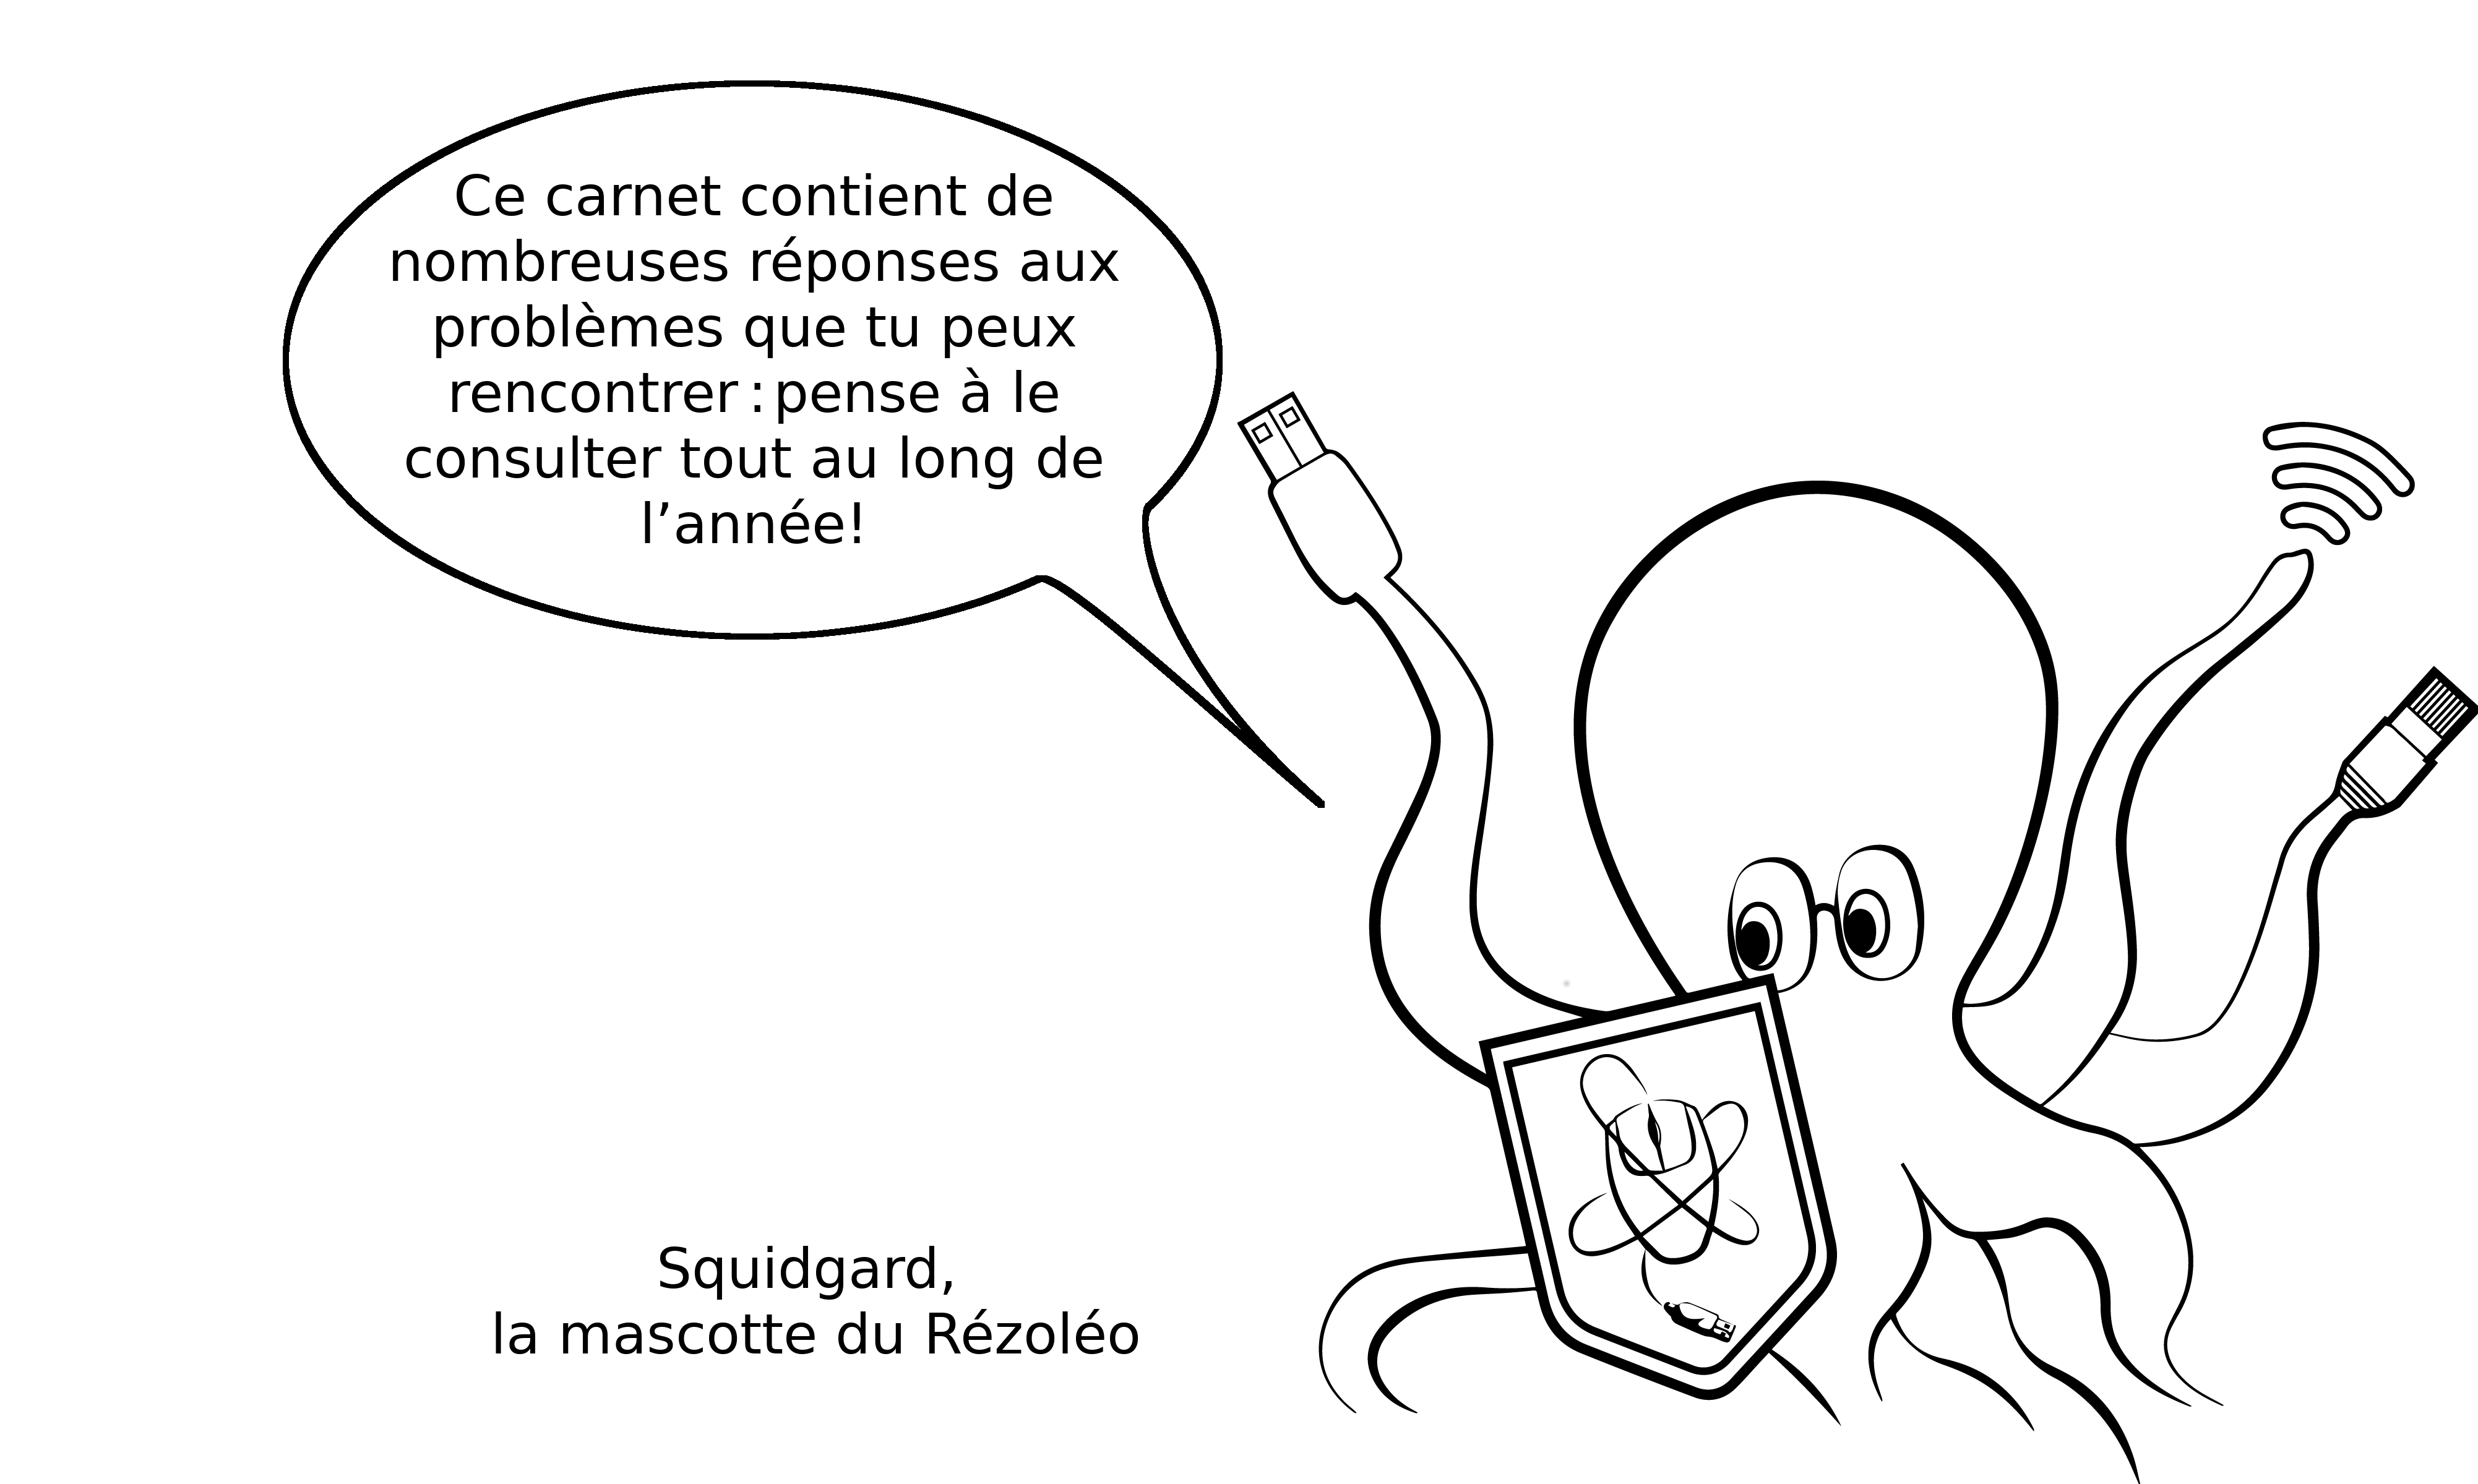
\includegraphics[scale=0.13]{imageAccueil.png}}
  \end{figure}

  \newpage
\section{Connexion internet}
  Chaque résident peut bénéficier d’une connexion Internet \footnote{Une connexion est associée à une personne (nom et chambre). Tu peux connecter au réseau plusieurs ordinateurs ainsi que te connecter librement depuis une chambre différente de la tienne.}. Pour être connecté, tu dois signer un contrat de connexion avec l’AGR  et le Rézoléo. Le prix de la connexion est de :
  {\begin{center}
    \textbf{8\EUR~par mois}
  \end{center}
  \centerline{ou}
  \begin{center}
    \textbf{80\EUR~par an}
  \end{center}

  Cette somme peut être payée par chèque à l’ordre du Rézoléo, en liquide ou par virement.
  \begin{description}
    \item \textbf{Filtrage et Censure}\vspace*{0.5cm} \newline Le Rézoléo ne filtre et ne censure aucun site web. Nous sommes tout de même soumis à la loi en ce qui concerne la surveillance des activités sur le réseau. Pour plus de détails voir :
    \begin{center}
      \verb|https://ri.rezoleo.fr|
    \end{center}
    \item \textbf{Se connecter pour la première fois}\vspace*{0.5cm} \newline Pour accéder à internet, viens au local du Rézoléo avec ton ordinateur ou ton routeur. Un membre de l’association permettra à ton appareil de rejoindre le réseau de la résidence. Si tu n'utilises pas de routeur, il te faudra un câble Ethernet (RJ45) pour te connecter dans ta chambre. Si tu n’en as pas, tu peux en acheter dans toutes les grandes surfaces, ou au Rézoléo.

  \end{description}

\section{Informations complémentaires}

  \subsection{Les Sites Indispensables}
    La vie centralienne s’organise autour de (trop) nombreux sites :
    \newline
    \begin{itemize}
      \item La boîte mail des anciens centraliens :
      \begin{center}
	\verb|https://mail.centraliens-lille.org|
      \end{center}
    \item Le planning en ligne, si tu veux aller en cours :
    \begin{center}
      \verb|https://planning.centralelille.fr|
    \end{center}
    \item Moodle, serveur pédagogique contenant tous les cours, pour réviser la veille des partiels : 
    \begin{center}
      \verb|https://moodle.centralelille.fr|
    \end{center}
    \item L’ENT, Environnement Numérique de Travail, regroupant divers services de Centrale : 
    \begin{center}
      \verb|https://ent.centralelille.fr|
    \end{center}
    \item Le poly online : Tous les tutos et infos des points suivants y sont expliqués et détaillés : 
    \begin{center}
      \verb|http://poly.rezoleo.fr|
    \end{center}
    \item Zimbra, la boîte mail interne de Centrale Lille :
    \begin{center}
      \verb|https://mail.ec-lille.fr/zimbra|
    \end{center}
    \item Absinthe, le site d'entraide scolaire des Centraliens :
    \begin{center}
      \verb|https://bde.rezoleo.fr/absinthe/|
    \end{center}
    \end{itemize}
  \subsection{La TNT via le réseau}
    Le réseau de la Rez’ permet de regarder les chaînes de la TNT directement sur ton ordinateur. Pour cela, il te faut un lecteur multimédia adapté, par exemple VLC.
    Tu peux alors accéder au dossier TNT dans la liste de lecture qui contient normalement toutes les chaînes de la TNT.
    \begin{description}
      \item \textbf{Comment y accéder?}\newline Accéder à la liste de lecture puis faire défiler 'Réseau local' sur la gauche. Cliquer sur 'Flux réseau (SAP)'.
    \end{description}
  \subsection{Stockage sur le serveur des élèves}
    Tu as la possibilité de bénéficier gratuitement du serveur des élèves pour tes sites d’assoces, de projet ou même de liste BDX. Pour en bénéficier, tu peux contacter le(la) Secrétaire acuel(le) du Rézoléo.
  \subsection{Les Mailing-lists}
    Une mailing-list, ou liste de diffusion, te permet de créer une adresse e-mail publique pour un groupe de personnes (par exemple, ton équipe projet, ou ton club).
    Pour créer une mailing-list en @lists.rezoleo.fr, envoye un mail au Rézoléo en précisant le nom de la mailing et l’adresse email de son administrateur.
  \subsection{Offres étudiantes}
    Etudiant à Centrale, tu as de nombreuses offres avantageuses chez plusieurs constructeurs (Apple, Dell, HP) ainsi que la possibilité d’avoir des licences de logiciels Microsoft gratuitement (Visual Studio, Office, Windows8 ou 10).
    Pour accéder à ces offres, identifie-toi sur l’ent, les offres sont visibles à l'accueil du site.
  \subsection{Réparation d'ordinateurs}
    Lorsque tu as un problème sur ton ordinateur, tu peux passer au Rézoléo pour le faire réparer. Si ton ordinateur est hors-d'usage, le PRI (le service informatique de Centrale) peut te prêter un ordinateur, le temps que tu t'en procures un autre. Leur bureau est au rez-de-chaussé du B7.
    \newpage
    \color{white}
      perdu!
    \newpage
    \color{black}
    \begin{figure}[h!]
      \centerline{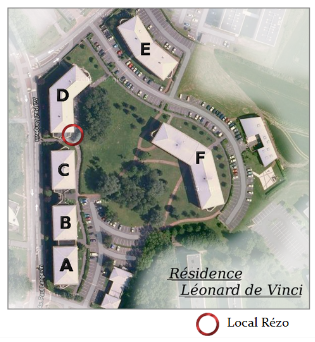
\includegraphics[scale=1]{carte.png}}
    \end{figure}
    Le \textbf{local Rézoléo} est ouvert tous les soirs pendant les 2 premières semaines de l``année. Ensuite, le local est ouvert les \textbf{lundi} et \textbf{vendredi soirs} de 18h à 20h.
    \begin{description}
      \vspace*{0.5cm}
      \item \textbf{Comment nous contacter?}\vspace*{0.5cm} \newline Tu peux nous envoyer un e-mail à l'adresse : \textbf{contact@rezoleo.fr}, ou passer au local lors des permanences.
    \end{description}
\end{document}